\documentclass[oneside]{article}[14pt]
\usepackage[left=2cm,right=2cm,top=2cm, bottom=2cm]{geometry} %margins
\usepackage{hyperref}
\hypersetup{colorlinks=true, linkcolor=blue, urlcolor=blue}

\usepackage{booktabs}
\usepackage{siunitx}
\setlength{\parindent}{0pt}
\setlength{\parskip}{10pt}
\usepackage{pdfpages}
\usepackage{svg}

\usepackage[T1]{fontenc}
\usepackage{graphicx, parskip, setspace, ragged2e, enumitem, times, amsmath, amssymb, amsthm, cancel, accents, tikz, tkz-euclide}
\graphicspath{ {assets/} }

\RaggedRight

\renewcommand{\labelenumi}{\arabic{enumi}.}
\renewcommand{\labelenumii}{(\alph{enumii})}
\renewcommand{\labelenumiii}{(\roman{enumiii})}

\title{\Huge{Vector Geometry, Calculus, Trigonometry}}
\author{\large{A set of questions curated by \textit{@icecreambobcat} from the NSWMaths Discord}}
\date{}

\everymath{\displaystyle}

\begin{document}
\newcommand{\HRule}{\rule{\linewidth}{0.5mm}}
\maketitle
\HRule
\vskip 2cm

\textbf{Question Credits:}
\begin{itemize}
	\item \href{https://nswmaths.com}{NSW Mathematics} (Most solutions can be found here)
  \item \textit{@moksifu} from the NSWMaths Discord
  \item \textit{@amiyuki7} from the NSWMaths Discord
  \item \textit{@magiicmushroom} from the NSWMaths Discord
  \item \textit{@oneeightseven} from the NSWMaths Discord
	\item SGS Mathematics Extension 1 Internals 2025
	\item JRAHS Mathematics Extension 1 Trial 2022
	\item NSB Mathematics Extension 1 Trial 2023
	\item NSB Mathematics Extension 1 Trial 2024
	\item SGHS Mathematics Extension 1 Trial 2023
\end{itemize}

\textbf{Question \& Mark Distribution:}
\begin{itemize}
	\item Vectors -- 7 questions; 24 marks
	\item Calculus -- 14 questions; 65 marks
	\item Trigonometry -- 5 questions; 21 marks
\end{itemize}

\vfill

{\LARGE{This is \textbf{NOT} intended to be completed under timed conditions; \\ any timing guides are a reference only.}}

\vfill
\HRule
\newpage

\section{Vectors}
\textit{Allow approximately 45 minutes for this section.} \\
\HRule \\
\vskip 4pt
\textbf{Question 1:}
Consider the points $A(-2,12)$, $B(2,8)$, $C(0,1)$ and $D(-5,0)$. There exists a unique square $PQRS$ such that each of the four points $A$, $B$, $C$ and $D$ lie on a different side of $PQRS$. \\
The \textbf{unit} vector in the direction of $\overrightarrow{PQ}$ is $\undertilde{u}=\begin{bmatrix} p \\ q \end{bmatrix}$, where $q$ and $p$ are positive, and the \textbf{unit} vector in the direction of $\overrightarrow{QR}$ is $\undertilde{v}$, as shown in the diagram below.
\begin{center}
	\begin{tikzpicture}[scale=0.8]
		\tkzDefPoint(-2.5, 6.5){P}
		\tkzDefPoint(2.5, 10.5){Q}
		\tkzDefPoint(6.5, 5.5){R}
		\tkzDefPoint(1.5, 1.5){S}

		\tkzDrawPolygon[semithick](P,Q,R,S)

		\tkzLabelPoint[above left](P){P}
		\tkzLabelPoint[above right](Q){Q}
		\tkzLabelPoint[below right](R){R}
		\tkzLabelPoint[below left](S){S}

		\tkzDefPointWith[linear,K=0.7](P,Q) \tkzGetPoint{A}
		\tkzDefPointWith[linear,K=0.5](Q,R) \tkzGetPoint{B}
		\tkzDefPointWith[linear,K=0.3](R,S) \tkzGetPoint{C}
		\tkzDefPointWith[linear,K=0.5](S,P) \tkzGetPoint{D}

		\tkzDrawPoint[thick](A) \tkzLabelPoint[above](A){A}
		\tkzDrawPoint[thick](B) \tkzLabelPoint[above right](B){B}
		\tkzDrawPoint[thick](C) \tkzLabelPoint[below](C){C}
		\tkzDrawPoint[thick](D) \tkzLabelPoint[left](D){D}

		\tkzDefPointWith[linear,K=0.33](P,Q) \tkzGetPoint{Q_third}
		\tkzDefPointWith[linear,K=0.33](Q,R) \tkzGetPoint{R_third}

		\tkzDrawSegment[->, very thick, >=Stealth](P,Q_third)
		\tkzLabelSegment[above left](P,Q_third){$\vec{u}$}

		\tkzDrawSegment[->, very thick, >=Stealth](Q,R_third)
		\tkzLabelSegment[above right](Q,R_third){$\vec{v}$}
	\end{tikzpicture}
\end{center}
\begin{enumerate}
	\item[(i)] Write down an expression for $\undertilde{v}$ in terms of $p$ and $q$. \hfill \fbox{\textbf{1}}
	\item[(ii)] Hence, calculate the exact area of $PQRS$. \hfill \fbox{\textbf{4}}
\end{enumerate}
\vskip 8pt

\textbf{Question 2:}
Define a sequence of vectors given by $T_0 = \mathbf{v}$ and $T_{n}$ is the vector from projecting $T_{n-1}$ onto $\mathbf{u}$. Prove by mathematical induction that for $n\geq 1$,
\[ T_n = \operatorname{proj}_{\mathbf u} \mathbf v .\]
\hfill \fbox{\textbf{3}}
\vskip 8pt

\textbf{Question 3:}
In triangle $OAB$, $M$ is the midpoint of $AB$ and $P$ internally divides $OB$ in the ratio $3:1$. $Q$ is the point on $AP$ such that $O, Q$ and $M$ are collinear. Find the ratio $OQ:QM$.
\hfill \fbox{\textbf{2}}
\newpage

\HRule \\
\vskip 4pt
\textbf{Question 4:}
Consider the unit circle around the origin $O$ in the diagram below, with $\undertilde{i}$ and $\undertilde{j}$ being the standard basis unit vectors in the horizontal and vertical directions respectively. The points $P$ and $Q$ lie on the unit circle such that $P$ is in the first quadrant and $Q$ is in the fourth quadrant. The angles $POX$ and $QOX$ have measures $\alpha$ and $\beta$ respectively, where $X$ is the point $(1,0)$. Let $\overrightarrow{OP} = \undertilde{p}$, $\overrightarrow{OQ}=\undertilde{q}$.
\begin{center}
	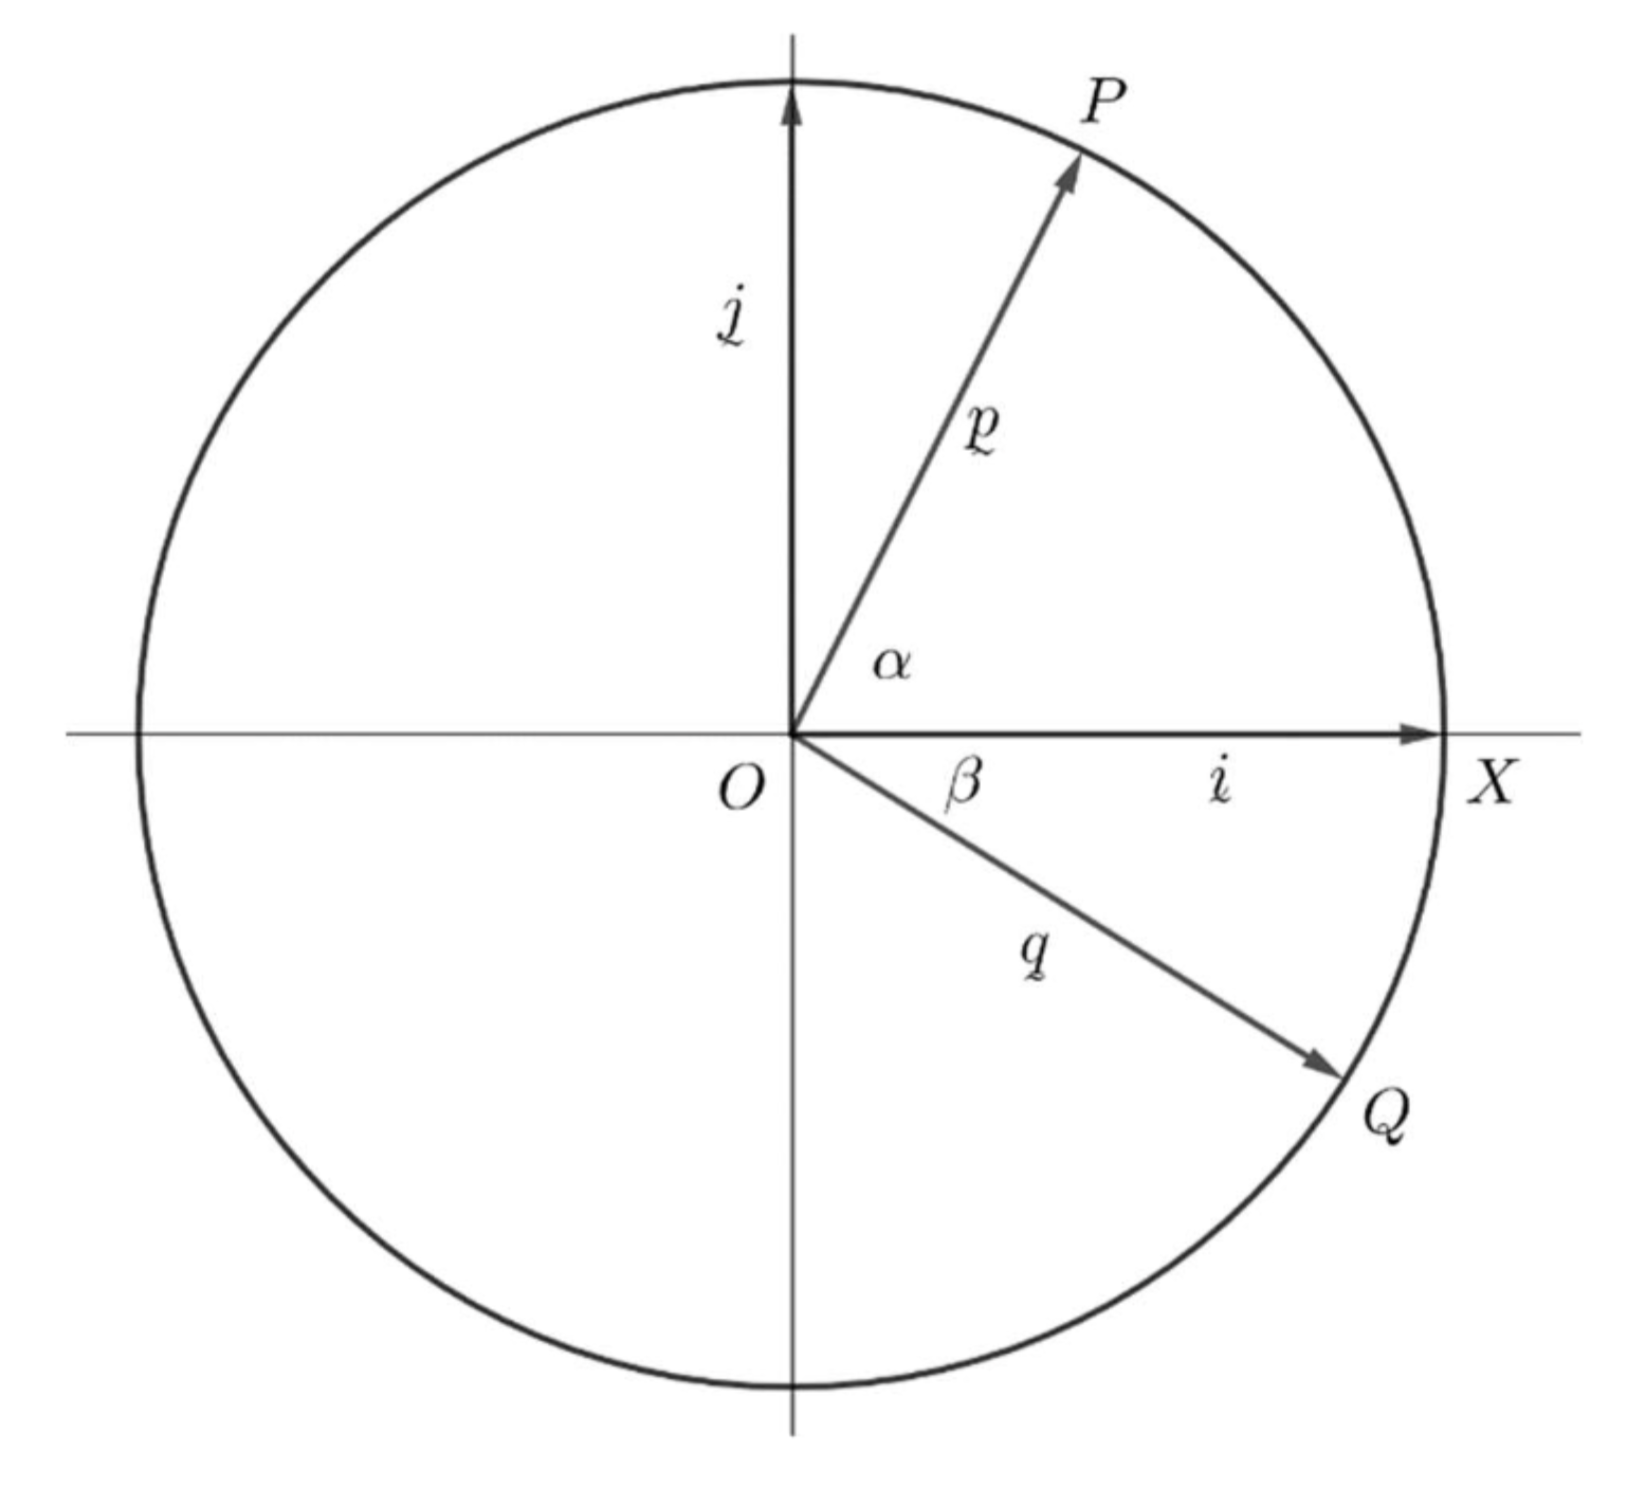
\includegraphics[width=0.5\textwidth]{s1q3.png}
\end{center}
\begin{enumerate}
	\item[(i)] Find $\undertilde{p}$ in terms of $\alpha$, and $\undertilde{q}$ in terms of $\beta$. \hfill \fbox{\textbf{2}}
	\item[(ii)] Hence, by considering $\undertilde{p}\cdot\undertilde{q}$, show that
	      \[\cos(\alpha+\beta) = \cos(\alpha)\cos(\beta) - \sin(\alpha)\sin(\beta)\]
	      \hfill \fbox{\textbf{2}}
\end{enumerate}
\vskip 8pt

\textbf{Question 5:}
Triangle $OAB$ is defined by two non-parallel and nonzero vectors $\overrightarrow{OA} = \undertilde{a}$ and $\overrightarrow{OB} = \undertilde{b}$. The angle between the vectors is $\theta$.
\begin{center}
	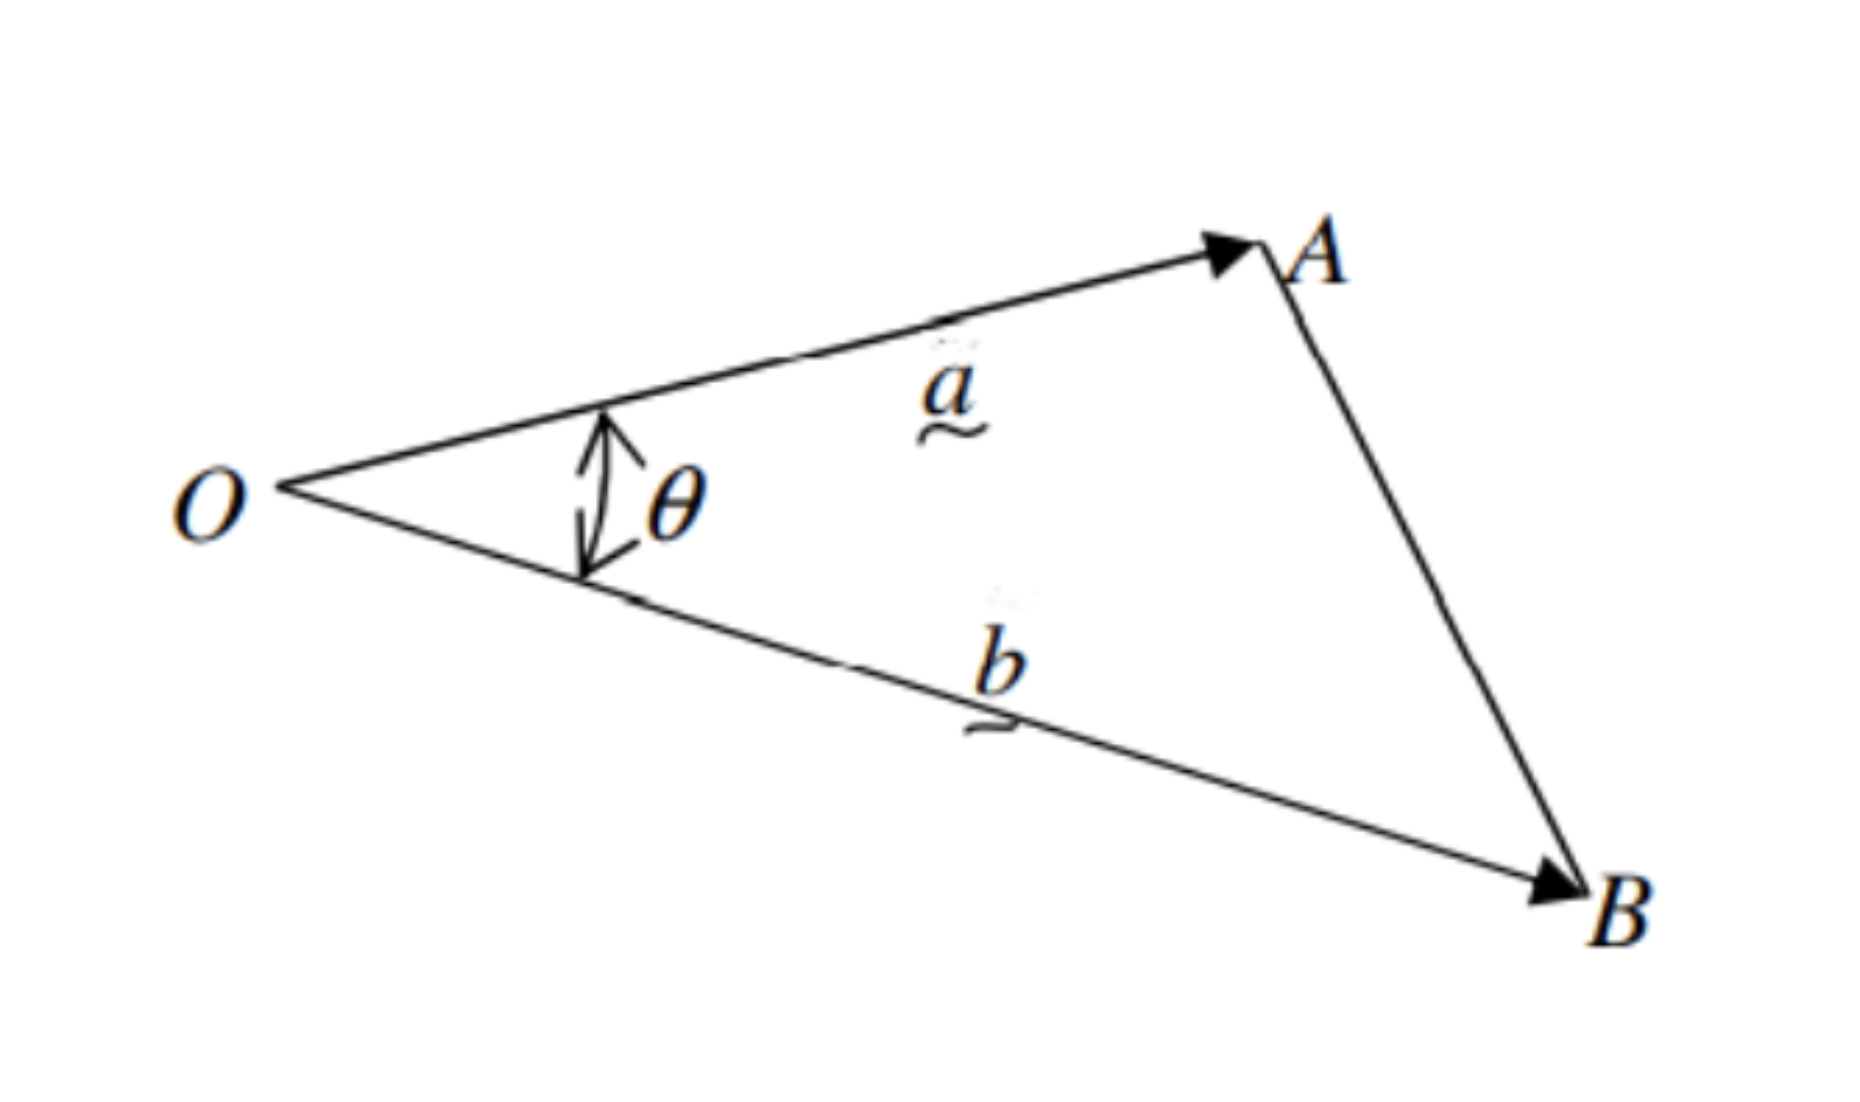
\includegraphics[width=0.5\textwidth]{s1q5.png}
\end{center}
Express the area of triangle $OAB$ in terms of dot products of $\undertilde{a}$ and $\undertilde{b}$. \hfill \fbox{\textbf{3}}
\newpage

\HRule \\
\vskip 4pt
\textbf{Question 6:}
The point $X$ is chosen within the interval $AB$ such that $AX:XB=m:n$, where $m$ and $n$ are positive and $m\neq n$. Let $\overrightarrow{OA}=\undertilde{a}$ and $\overrightarrow{OB}=\undertilde{b}$, as shown.
\begin{center}
	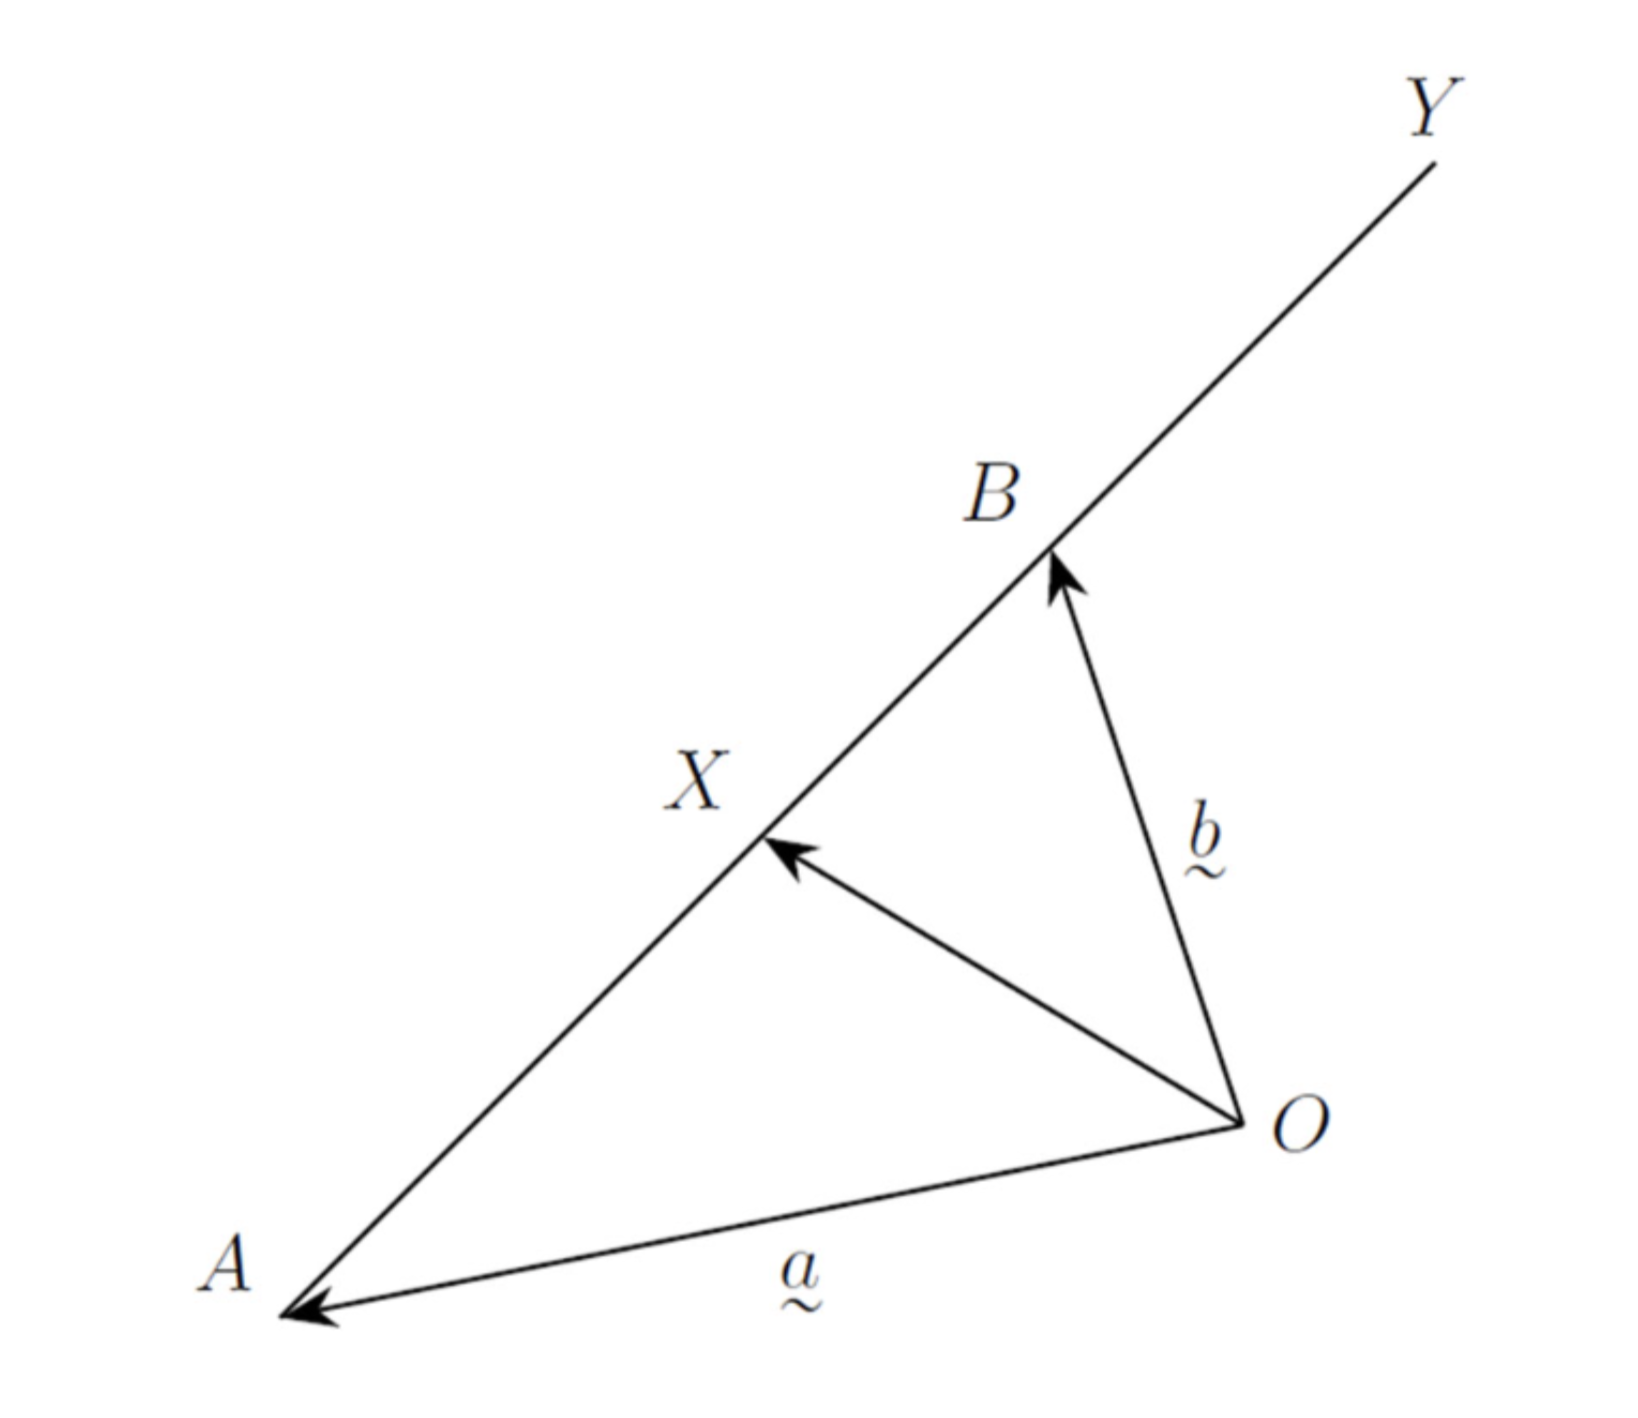
\includegraphics[width=0.6\textwidth]{s1q6.png}
\end{center}
\begin{enumerate}
	\item[(i)] Show that $\overrightarrow{OX}=\dfrac{n\undertilde{a}+m\undertilde{b}}{m+n}$. \hfill \fbox{\textbf{2}}
	\item[(ii)] The point $Y$ is on the line $AB$ such that
	      \[\overrightarrow{OY}=\dfrac{n\undertilde{a}-m\undertilde{b}}{m-n}. \tag{Do \textbf{not} prove this}\]
	      If $OX$ is perpendicular to $OY$, show that $n|\undertilde{a}|=m|\undertilde{b}|$. \hfill \fbox{\textbf{2}}
\end{enumerate}
\newpage

\HRule \\
\vskip 4pt
\textbf{Question 7:}
The spiral $\mathcal{S}$ is defined by the parametric vector \[\undertilde{r}(\theta)=\begin{pmatrix} ae^{k\theta}\cos\theta \\ ae^{k\theta}\sin\theta \end{pmatrix}\] for $a, k \in \mathbb{R}^+$. \\
The \textit{pitch angle}, $\alpha$, at any point $P$ on $\mathcal{S}$ is the angle between the tangent to the circle centered at $O$ with radius $|\overrightarrow{OP}|$, and the tangent to $\mathcal{S}$ at $P$. \\
\begin{center}
  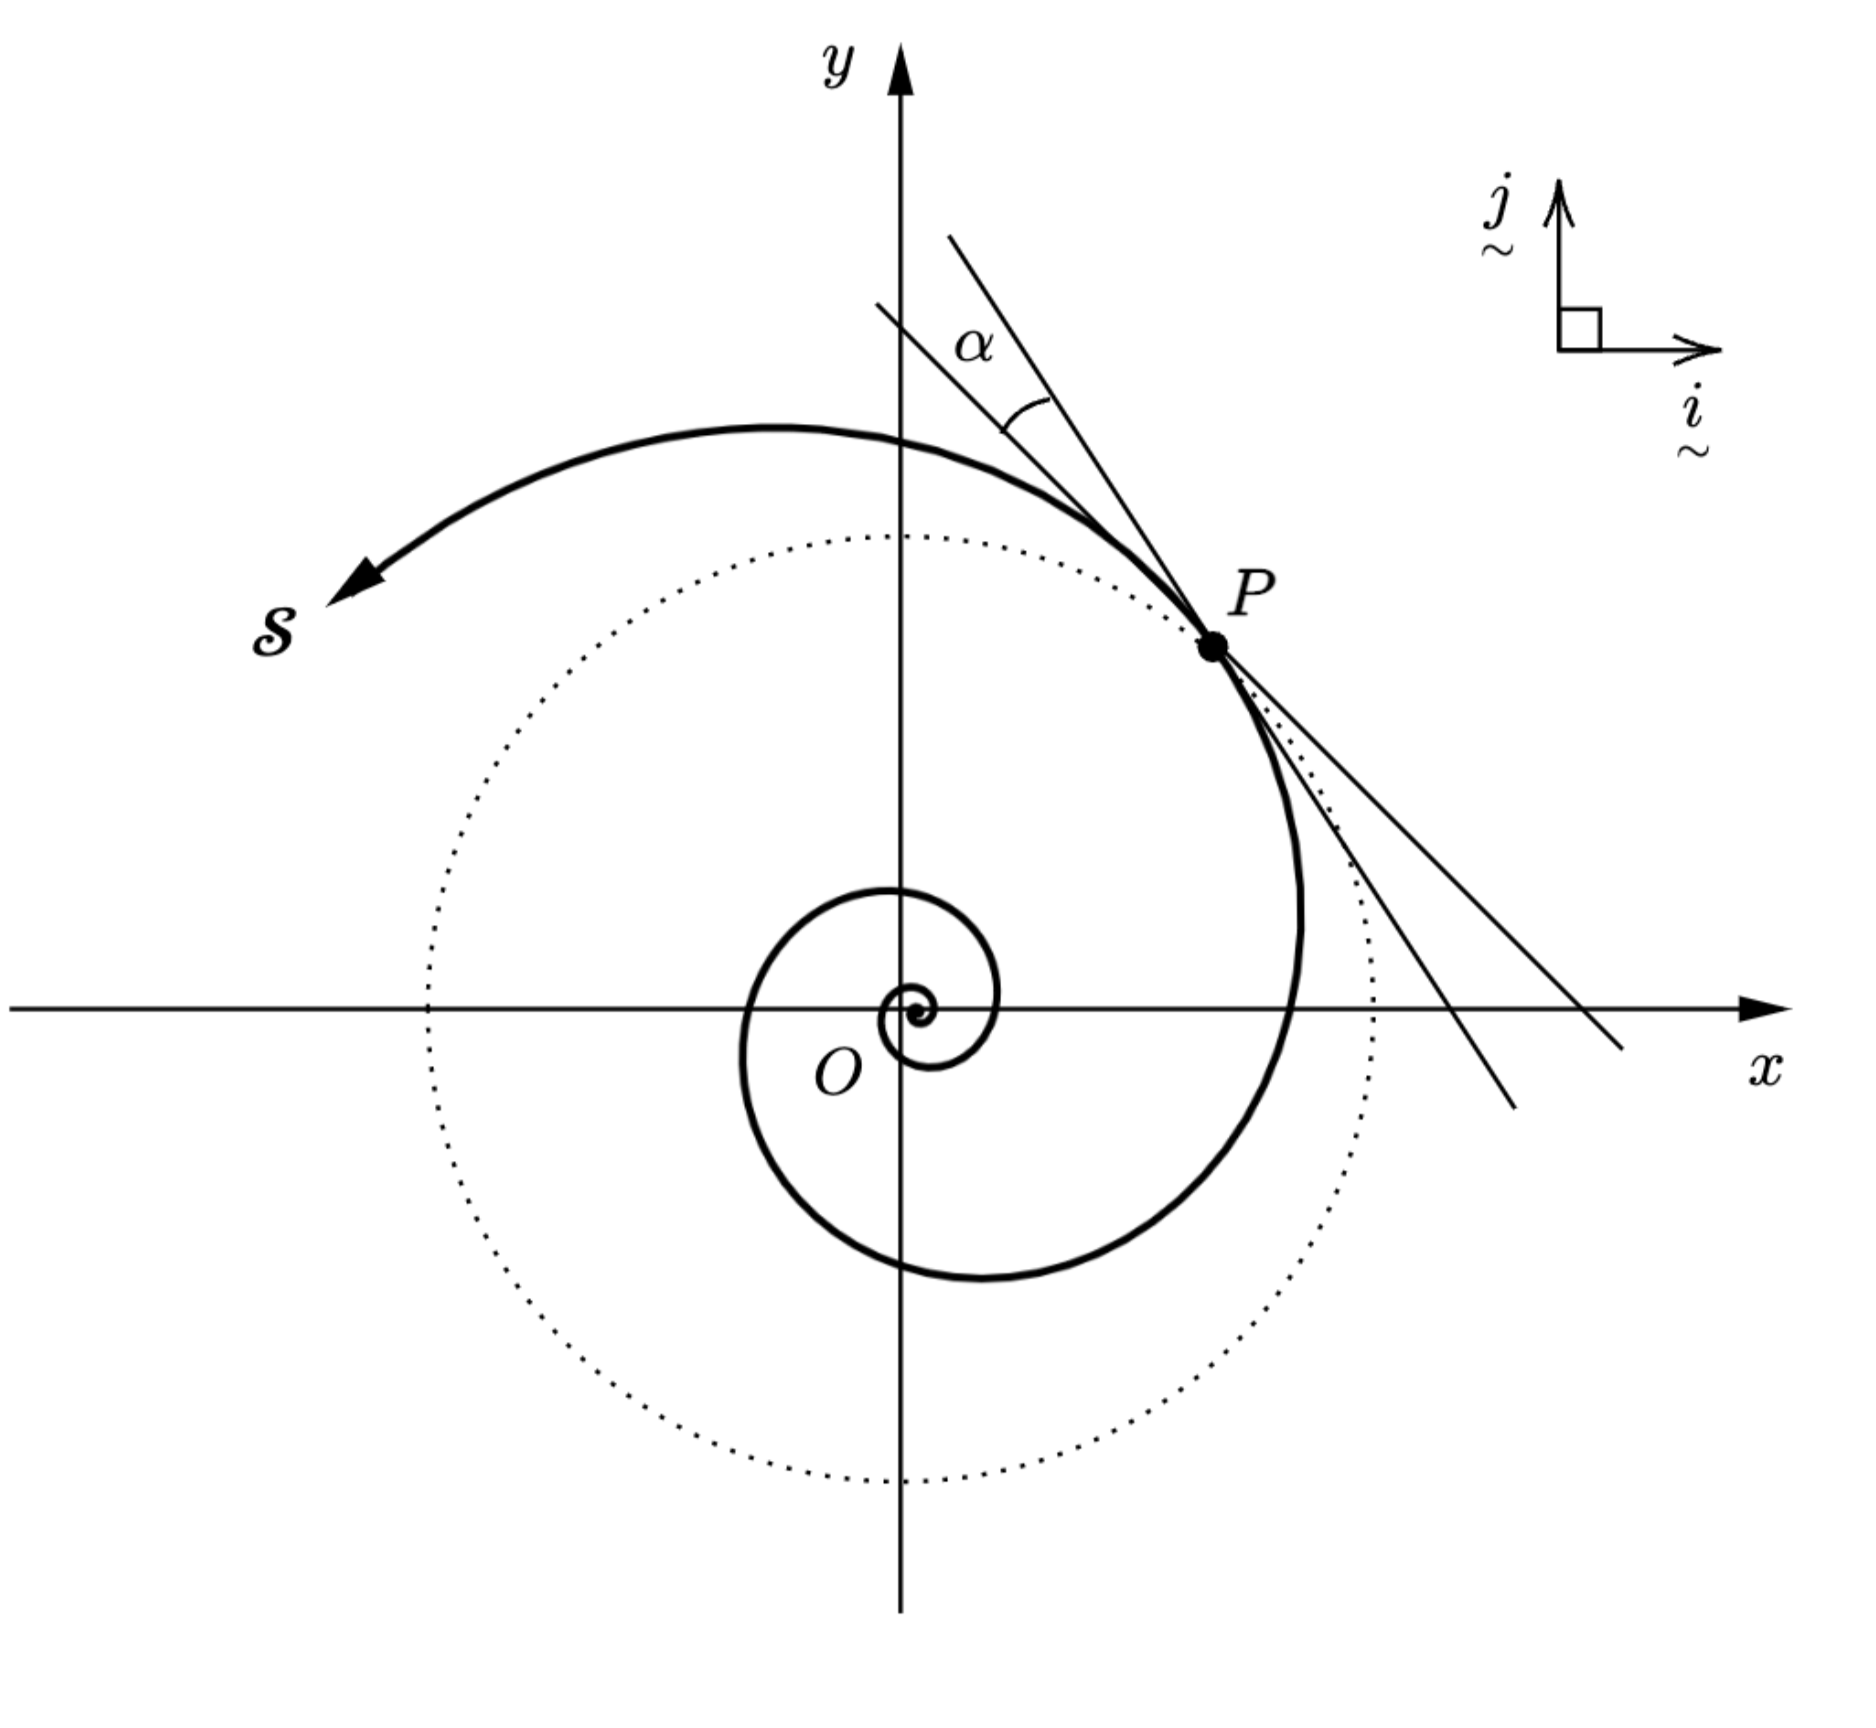
\includegraphics[width=0.6\textwidth]{s1q7.png}
\end{center}
Prove $\tan\alpha=k$. \hfill \fbox{\textbf{3}}

\newpage

\section{Calculus}
\textit{Allow approximately 120 minutes for this section.} \\
\HRule \\
\vskip 4pt
\textbf{Question 1:}
Six points $P_1$, $P_2$, $P_3$, $P_4$, $P_5$ and $P_6$ form the vertices of a regular hexagon $H_1$. An animated program is rotating these six points at a constant speed of 3 cm/s around the perimeter of another regular hexagon, $H_2$, which has a side length of 20cm.
\begin{center}
	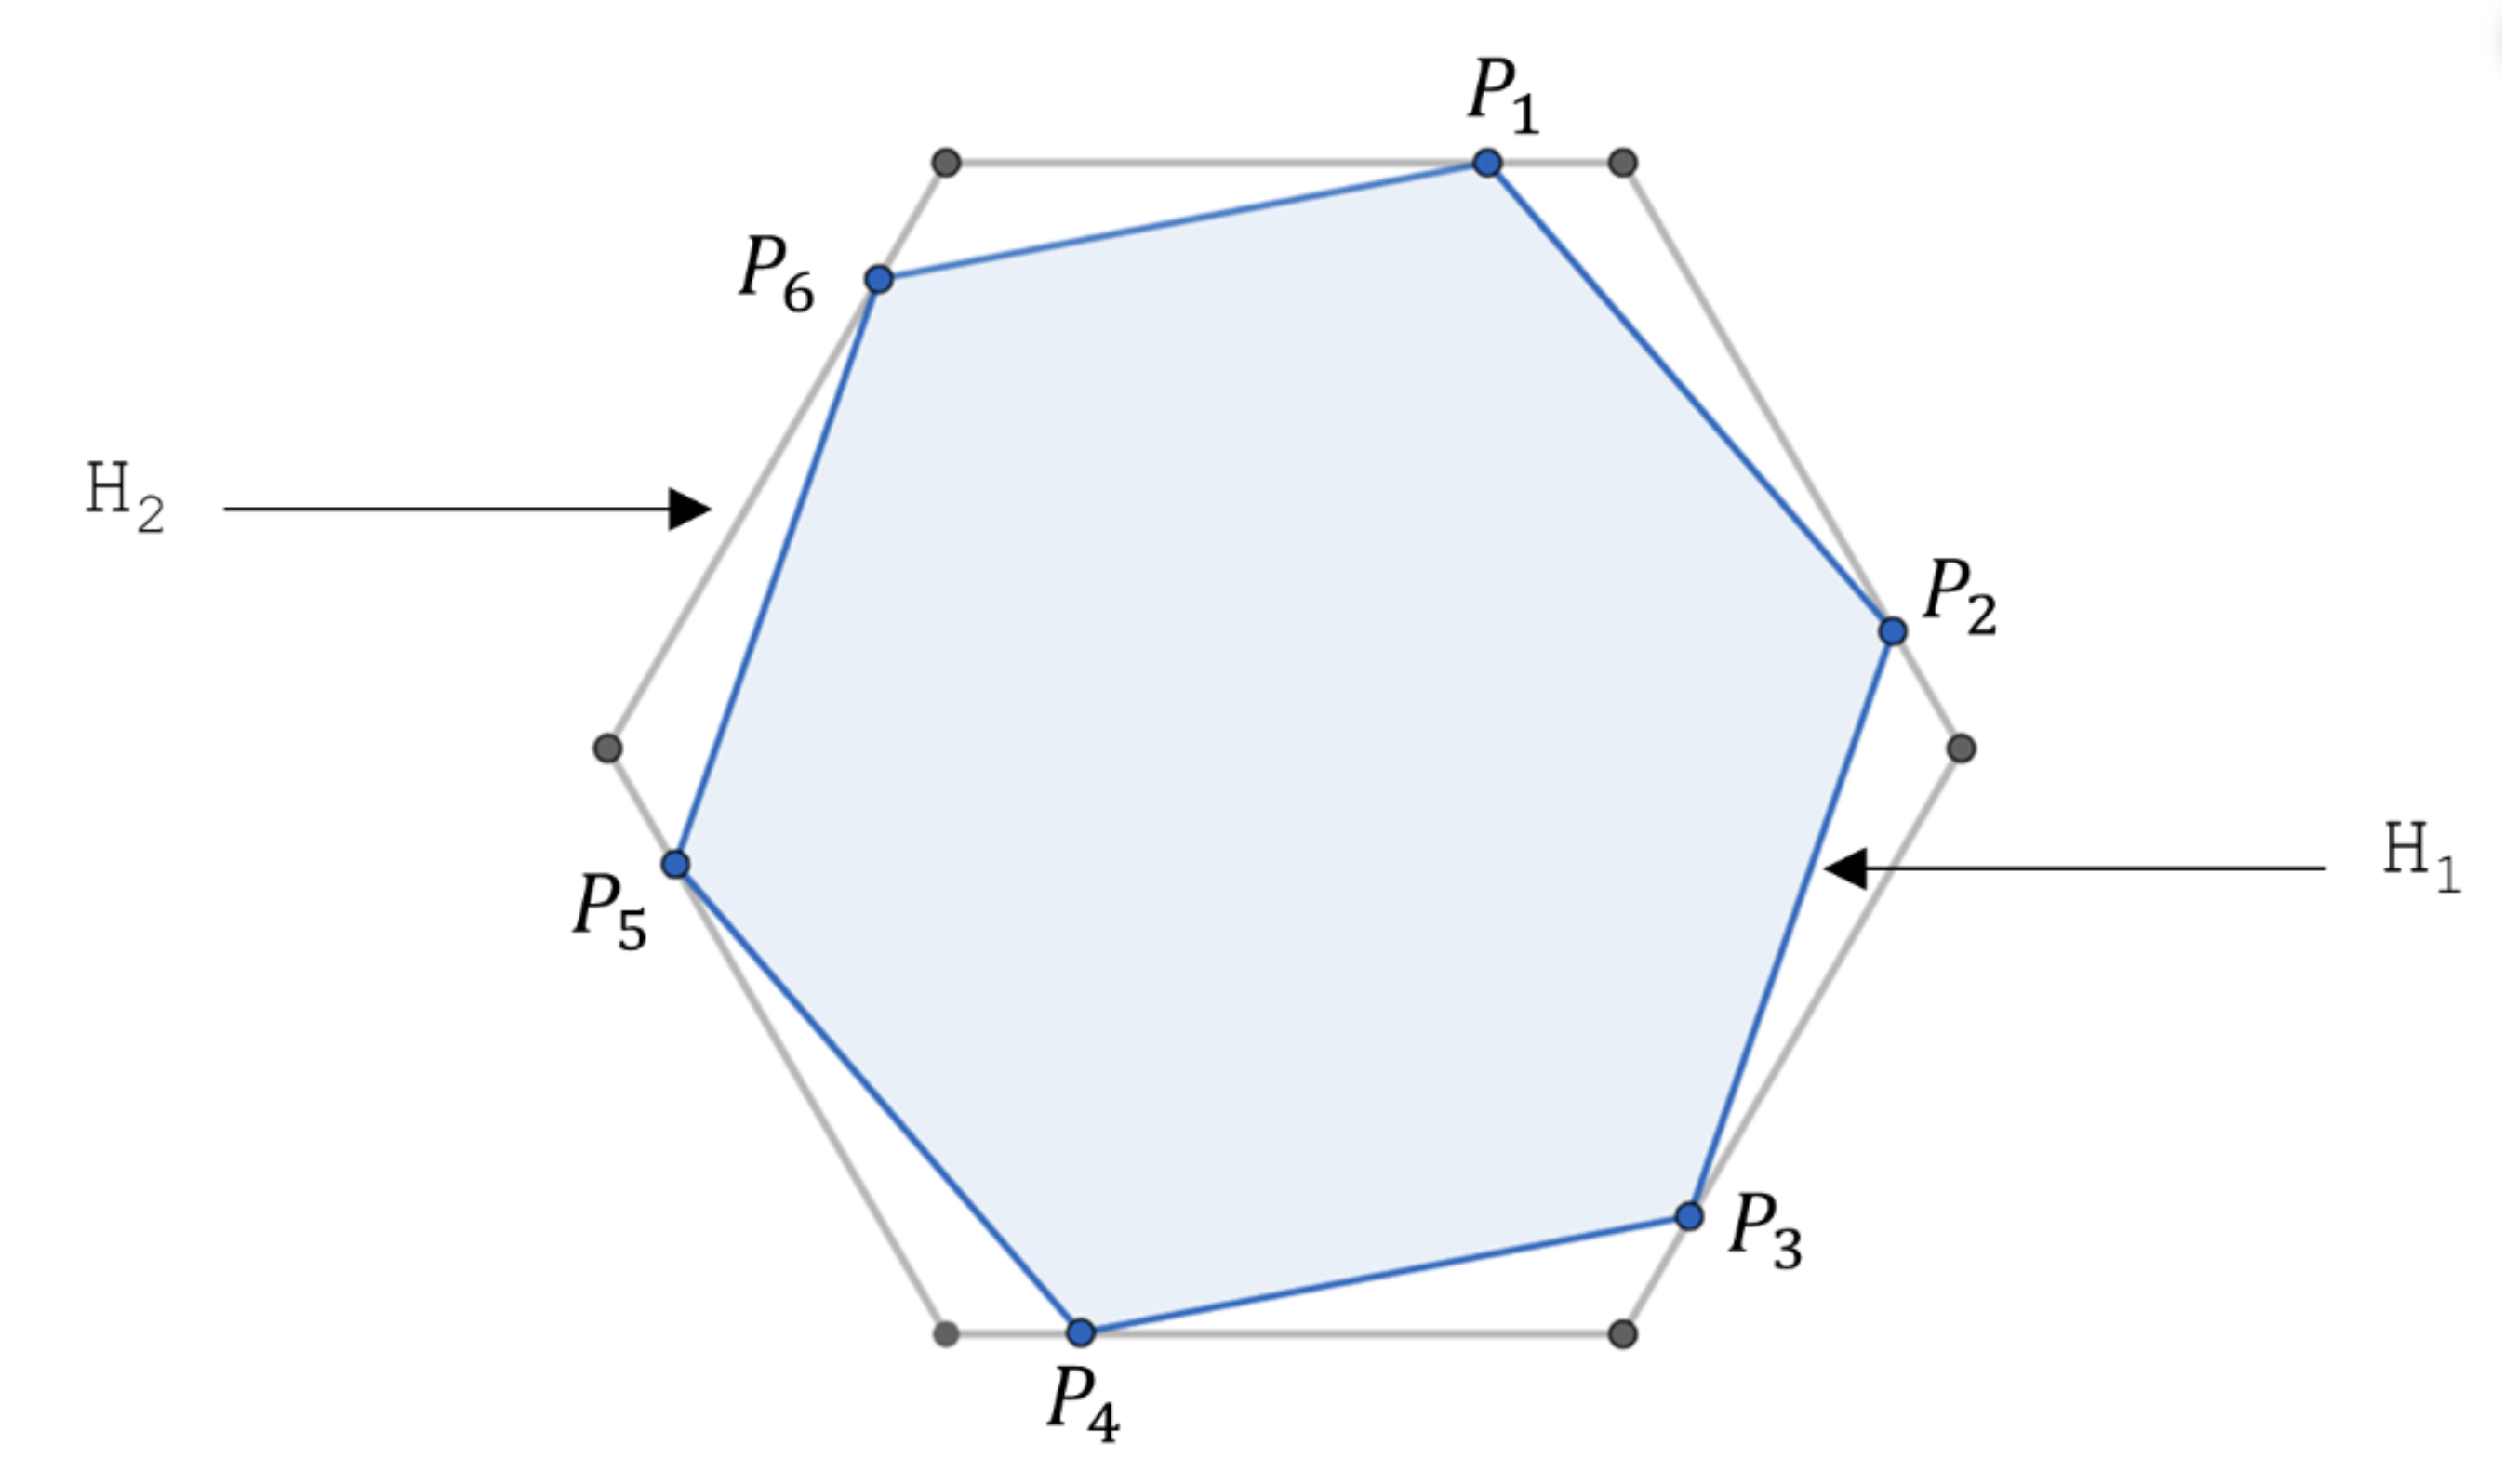
\includegraphics[width=0.8\textwidth]{s2q1.png}
\end{center}
Initially, the six vertices of $H_1$ lie on top of the six vertices of $H_2$. Determine the rate of change of the area $H_1$ ten seconds after the animation begins. \hfill \fbox{\textbf{4}}
\vskip 8pt

\textbf{Question 2:}
Consider the quadratic function $f(x)=px^2+qx+r$.\\

The points $A(a,f(a))$ and $B(b,f(b))$ lie on the graph $y=f(x)$. The secant line $\ell_S$ passes through $A$ and $B$. It is known that there exists a unique line $\ell_T$ that is parallel to $\ell_S$, and tangent to the graph $y=f(x)$ at the point $C(c,f(c))$. (Do \textbf{not} prove the existence of $\ell_T$).
\begin{enumerate}
	\item[(i)] Prove that $c=\dfrac{a+b}{2}$. \hfill \fbox{\textbf{1}}
	\item[(ii)] The lines $\ell_S$, $\ell_T$, $x=a$, and $x=b$ enclose a parallelogram region. Prove that the area of this region is \[\left\lvert\frac{p(a-b)^3}{4}\right\rvert.\] \hfill \fbox{\textbf{3}}
	\item[(iii)] Hence, or otherwise, prove that the area of $\bigtriangleup ABC$ is $\dfrac{3}{4}$ of the area enclosed by $\ell_S$ and the graph $y=f(x)$. \hfill \fbox{\textbf{4}}
\end{enumerate}
\newpage

\HRule \\
\vskip 4pt
\textbf{Question 3:}
The graph of $f(x)=2+\sin x+\cos 3x$ is shown below.

Let $g(t)$ be the area under the graph $y=f(x)$ on the interval $\left[t,t+\dfrac{\pi}{2}\right].$
\begin{center}
	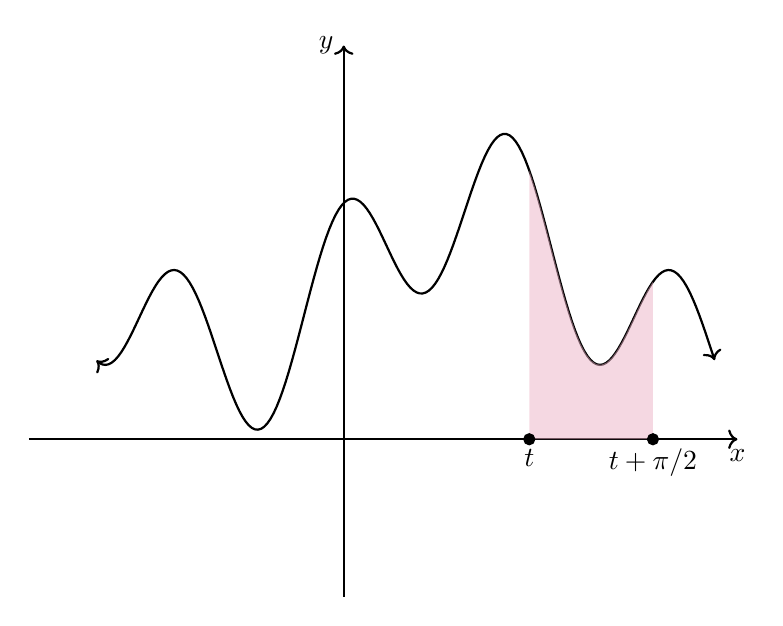
\begin{tikzpicture}
		\draw [thick] [->] (-4,0)--(5,0) node[right, below] {$x$};

		\draw [thick] [->] (0,-2)--(0,5) node[above, left] {$y$};

		\draw [domain=-pi:1.5*pi, samples=200, variable=\x, black, thick, <->] plot ({\x}, {2 + cos(deg(3*\x)) + sin(deg(\x))});

		\fill [purple!30, opacity=0.5, domain=3*pi/4:3*pi/4+pi/2, variable=\x]
		(3*pi/4, 0)
		-- plot ({\x}, {2 + cos(deg(3*\x)) + sin(deg(\x))})
		-- (3*pi/4+pi/2, 0);

		\filldraw [black] (3*pi/4,0) circle (2pt) node[below] {$t$};
		\filldraw [black] (3*pi/4+pi/2,0) circle (2pt) node[below] {$t+\pi/2$};
	\end{tikzpicture}
\end{center}
\begin{enumerate}
	\item[(i)] Show that
	      \[g(t)=\pi+\sqrt{2}\left(\sin\left(t+\dfrac{\pi}{4}\right)-\dfrac{1}{3}\sin\left(3t+\dfrac{\pi}{4}\right)\right).\] \hfill \fbox{\textbf{3}}
	\item[(ii)] Hence, find the exact maximum area of a $\dfrac{\pi}{2}$-wide slice. \hfill \fbox{\textbf{3}}
\end{enumerate}
\vskip 8pt

\textbf{Question 4:}
Show, using calculus, that for $x>0$, $$\ln(1+x)-x+\dfrac{x^2}{2}<\dfrac{x^3}{3}.$$ \hfill \fbox{\textbf{3}}
\vskip 8pt

\textbf{Question 5:}
Let $p(x), q(x)$ and $r(x)$ be polynomials. Let
\[ F(x) = \left( \int_1^x p(t)\mathrm dt\right) \left( \int_1^x q(t) \mathrm dt \right)\left(\int_1^x r(t) \mathrm dt\right).\]

Show that if the degree of $F(x)$ is at least 3, then $(x-1)^3$ is a factor of $F(x)$. \hfill \fbox{\textbf{4}}
\vskip 8pt

\textbf{Question 6:}
Suppose $m$ and $n$ are non-negative integers such that $m < n$. Using the substitution $u = \tan x$, show that

\[
	\int_{0}^{\frac{\pi}{4}} \frac{\sin^{2m} x}{\cos^{2n} x} \,dx =
	\sum_{k=0}^{n-m-1} \binom{n-m-1}{k} \frac{1}{2k + 2m + 1}.
\]
\hfill \fbox{\textbf{4}}
\newpage

\HRule \\
\vskip 4pt
\textbf{Question 7:}
A differentiable function $f$ satisfies the equation \[f(x)=x\int_1^x f(t)\,dt.\]

\begin{enumerate}
	\item[(i)] Explain why $f(1)=0$. \hfill \fbox{\textbf{1}}
	\item[(ii)] Find all $f$. \hfill \fbox{\textbf{2}}
\end{enumerate}
\vskip 8pt

\textbf{Question 8:}
Given \[f(x)=\dfrac{e^x-e^{-x}}{e^x+e^{-x}},\]
\begin{enumerate}
	\item[(i)] Show that $f(x)$ has no stationary points. \hfill \fbox{\textbf{2}}
	\item[(ii)] Given that $y\pm 1$ are horizontal asymptotes, sketch the curve. \hfill \fbox{\textbf{2}}
	\item[(iii)] For $k>0$, consider the area enclosed by the curve, the lines $y=1$, $x=0$, and $x=k$. Show that this area can be expressed in the form \[\ln\left(\dfrac{2e^k}{e^k+e^{-k}}\right).\] \hfill \fbox{\textbf{2}}
	\item[(iv)] Hence, justify why for all values of $k$, the area found in part (iii) is always less than 2. \hfill \fbox{\textbf{1}}
\end{enumerate}
\vskip 8pt

\textbf{Question 9:}
By using the substitution $u=\tan^{-1}x$, evaluate $\int\dfrac{e^{\tan^{-1}x}}{1+x^2}\,dx$. \hfill \fbox{\textbf{3}}
\vskip 8pt

\textbf{Question 10:}
The diagram shows a region bound by the curve $C$ with the equation $y=3^x$, the line $l$, and the $x$-axis. The x coordinates of points $P$ and $Q$ are $2$ and $\left(2-\dfrac{1}{\ln 3}\right)$ respectively.
\begin{center}
	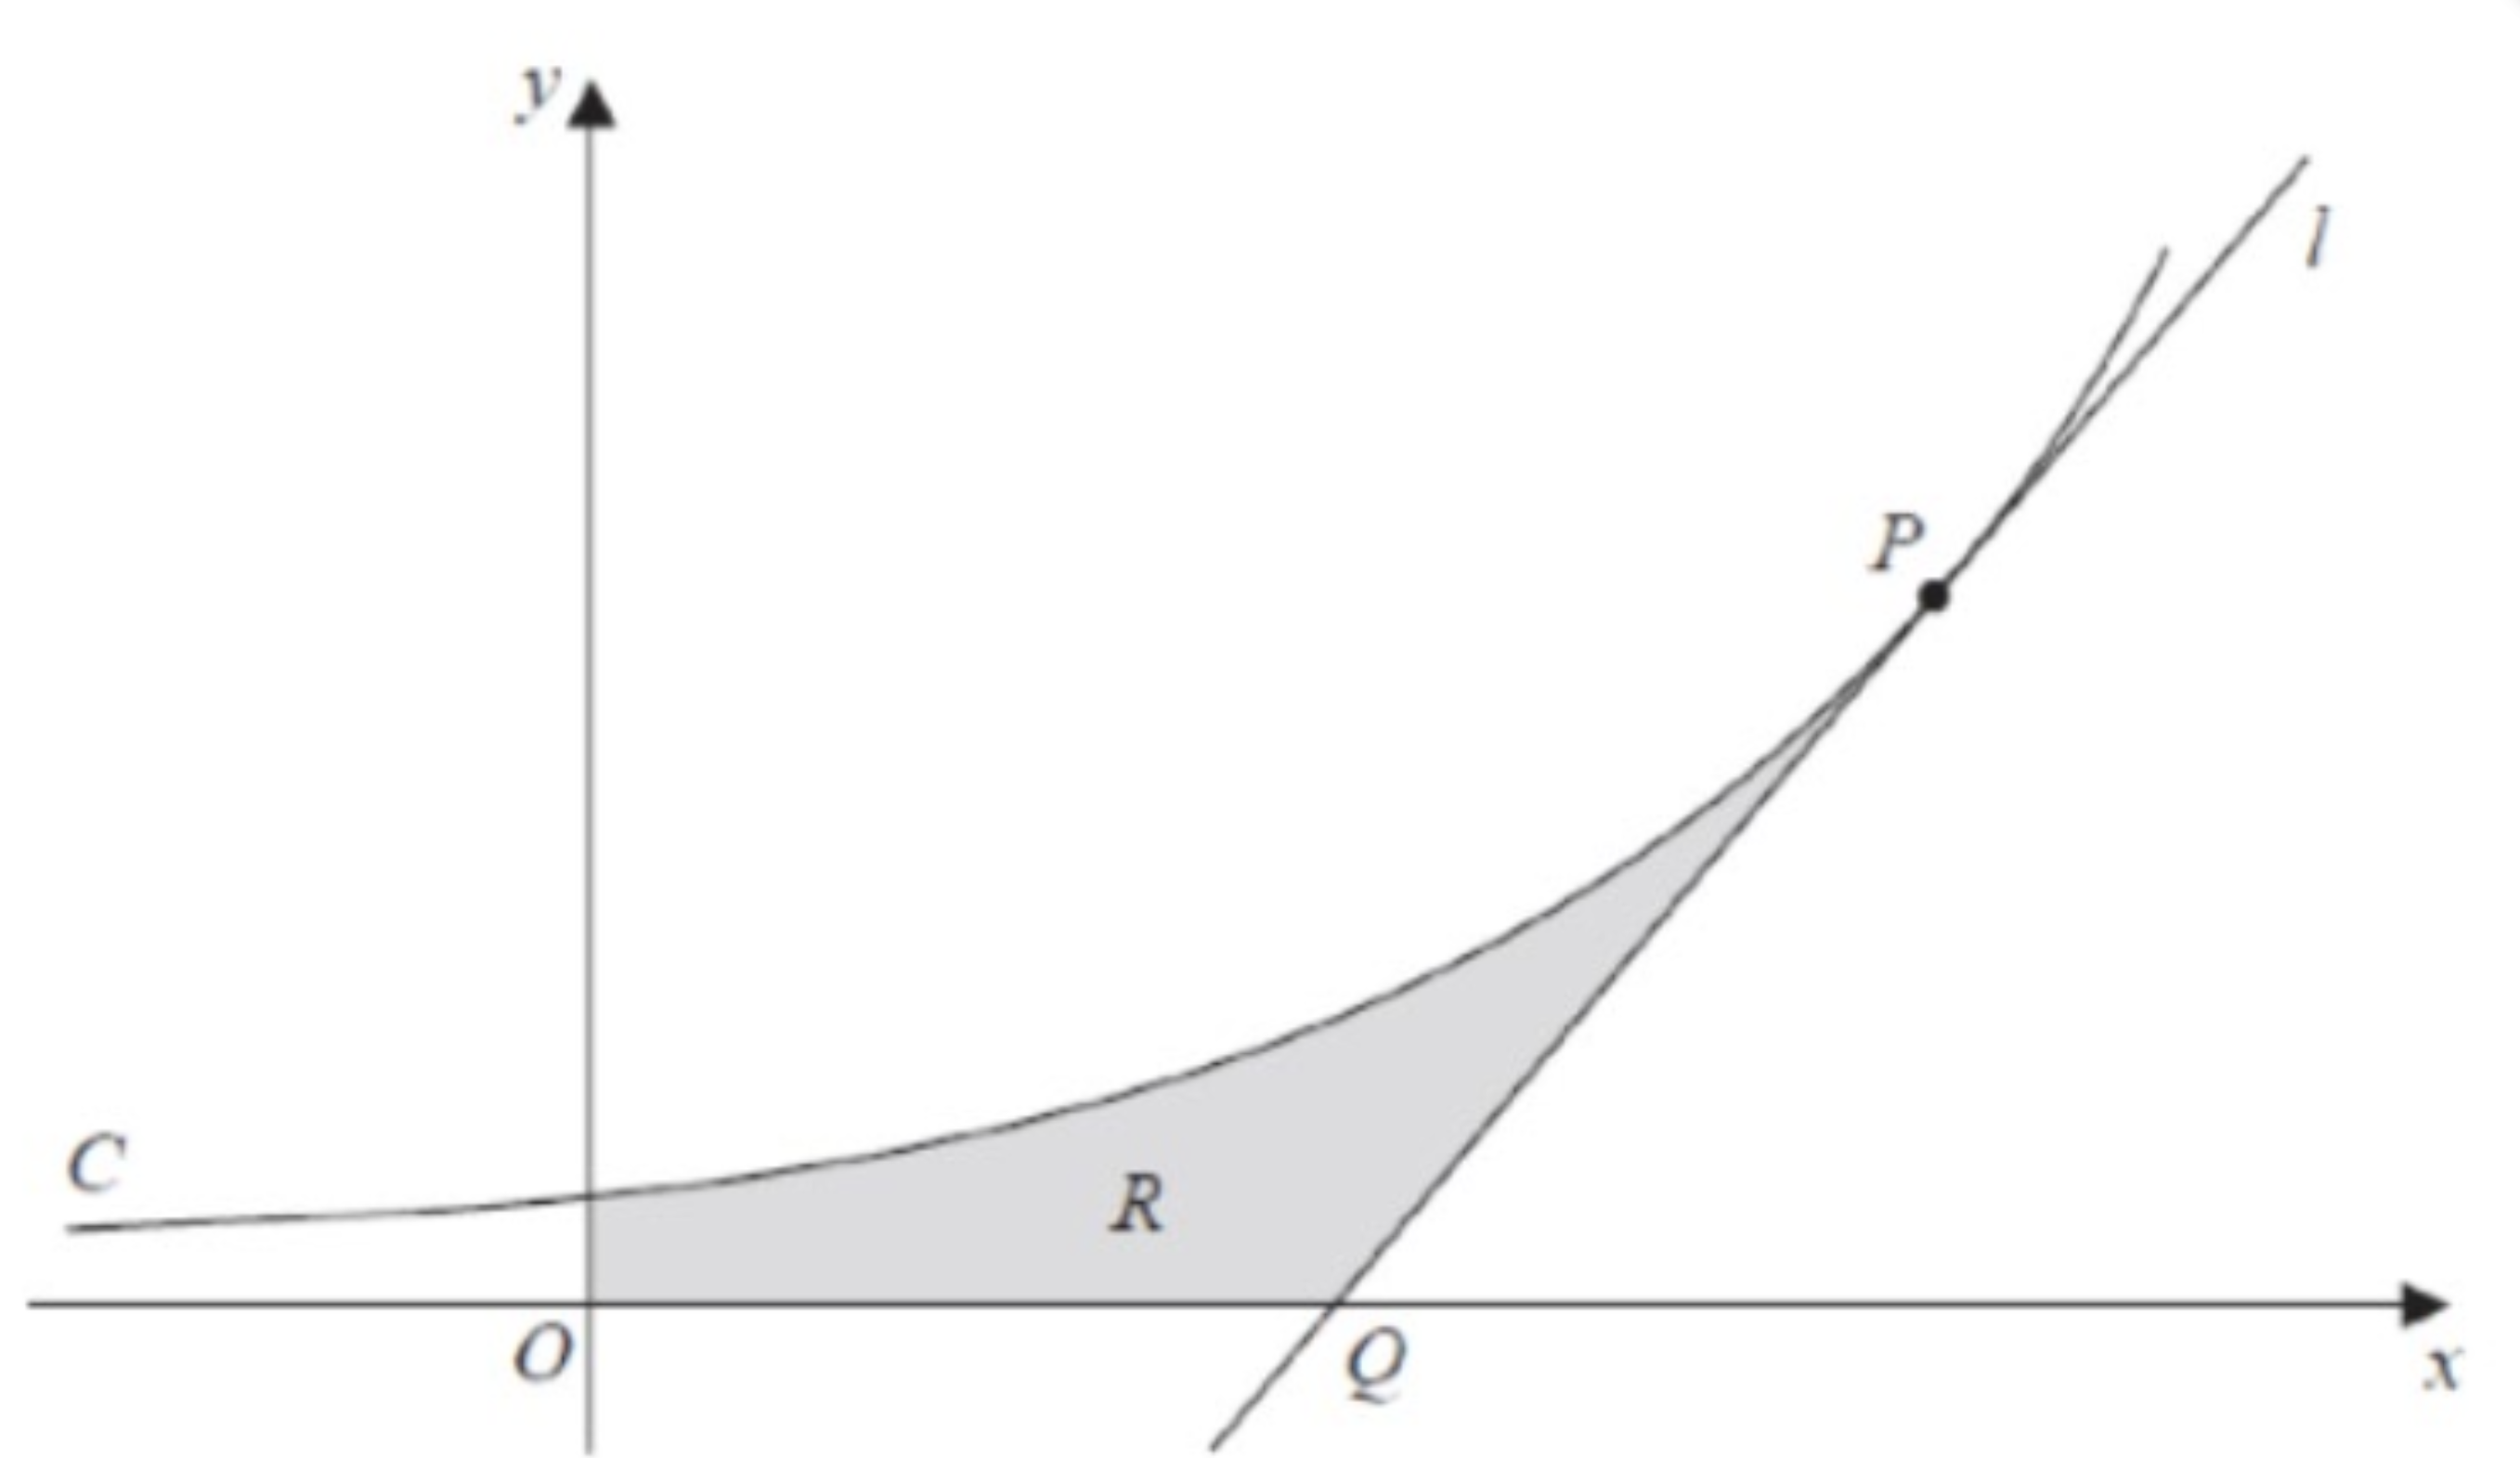
\includegraphics[width=0.6\textwidth]{s2q10.png}
\end{center}
A solid is created when the region $R$ is revolved around the $x$ axis. Find the volume of the solid formed. \hfill \fbox{\textbf{4}}
\newpage

\HRule \\
\vskip 4pt
\textbf{Question 11:}
A hemi-spherical bowl has a radius of 3m. Oil is poured in at a constant rate of $\dfrac{\pi}{3}\mathrm{m}^3/\mathrm{min}$.
\begin{enumerate}
	\item[(i)] Show that when the depth of the oil is $h$ metres, the volume of oil is given by \[V=\dfrac{\pi}{3}(9h^2-h^3).\] \hfill \fbox{\textbf{2}}
	\item[(ii)] Show that the depth of the oil in the bowl after 8 minutes is 1 meter. \hfill \fbox{\textbf{3}}
	\item[(iii)] At what rate is $h$ increasing at this time? \hfill \fbox{\textbf{2}}
\end{enumerate}
\vskip 8pt

\textbf{Question 12:}
\begin{enumerate}
	\item[(i)] By equating coefficients, find the values of $P$ and $Q$ such that \[P(2\sin x + \cos x) + Q(2\cos x - \sin x) \equiv 7\sin x + 11\cos x.\] \hfill \fbox{\textbf{2}}
	\item[(ii)] Hence, or otherwise, evaluate \[\int_0^{\frac{\pi}{2}}\dfrac{7\sin x + 11\cos x}{2\sin x + \cos x}\,dx.\] \hfill \fbox{\textbf{2}}
\end{enumerate}
\vskip 8pt

\textbf{Question 13:}
Evaluate:
\begin{enumerate}
	\item[(i)] \[\int\dfrac{\sin x}{\sin x + \sec x}\,dx.\] \hfill \fbox{\textbf{3}}
	\item[(ii)] \[\int\dfrac{dx}{2+\tan^2x}.\] \hfill \fbox{\textbf{2}}
\end{enumerate}
\vskip 8pt

\textbf{Question 14:}
Show that \[\int^{-\frac{2}{5}}_{-\frac{6}{5}}\dfrac{\sqrt{25x^2-4}}{x}\,dx=\pi-4\sqrt{2}-2\sin^{-1}\left(\dfrac{1}{3}\right).\] \hfill \fbox{\textbf{3}}
\newpage

\section{Trigonometry}
\textit{Allow approximately 45 minutes for this section.} \\
\HRule \\
\vskip 4pt
\textbf{Question 1:}
Consider the equation $$\dfrac{\sqrt{3}-1}{\sin x}+\dfrac{\sqrt{3}+1}{\cos x}=4\sqrt 2$$ for $0<x<\dfrac{\pi}{2}$. It is given that $\sin\left(\dfrac{\pi}{12}\right)=\dfrac{\sqrt{6}-\sqrt{2}}{4}$ and $\cos\left(\dfrac{\pi}{12}\right)=\dfrac{\sqrt{6}+\sqrt{2}}{4}$.
\begin{enumerate}
	\item[(i)] Verify that $x=\dfrac{\pi}{12}$ is a solution to the equation. \hfill \fbox{\textbf{1}}
	\item[(ii)] Hence, find the other solution to the equation for $0<x<\dfrac{\pi}{2}$. \hfill \fbox{\textbf{3}}
\end{enumerate}
\vskip 8pt

\textbf{Question 2:}
Consider the polynomial equation $x^3-5x^2-12x+8=0$.
\begin{enumerate}
	\item[(i)] Show that the equation has exactly one negative root, and two positive roots. \hfill \fbox{\textbf{2}}
	\item[(ii)] Let the roots of the equation be $\tan\alpha$, $\tan\beta$ and $\tan\gamma$, where $\alpha,\beta,\gamma \in \left(-\frac{\pi}{2},\frac{\pi}{2}\right)$.

	      Justify, with appropriate calculations and reasoning, why\[\alpha + \beta + \gamma = \frac{\pi}{4}.\] \hfill \fbox{\textbf{3}}
\end{enumerate}
\vskip 8pt

\textbf{Question 3:}
Solve the following equation for $x$, giving your answer as exact values: \[ \sin\left(2\cos^{-1}\left(\cot\left(2\tan^{-1}(x)\right)\right)\right)=0.\] \hfill \fbox{\textbf{2}}
\vskip 8pt

\textbf{Question 4:}
Let $\theta$ be the measure of an acute angle.
\begin{enumerate}
	\item[(i)] Using a suitable expansion of $\sin 6\theta$, show that \[(\sin 2\theta)^3-\dfrac{3}{4}\sin 2\theta + \dfrac{1}{4}\sin 6\theta = 0.\] \hfill \fbox{\textbf{2}}
	\item[(ii)] If $x=4\sin 2\theta$ and $x^3-12x+8=0$, show that $\sin 6\theta = \dfrac{1}{2}$. \hfill \fbox{\textbf{1}}
	\item[(iii)] Using the result in (ii), evaluate \[\left(\sin\dfrac{\pi}{18}\right)^2+\left(\sin\dfrac{13\pi}{18}\right)^2+\left(\sin\dfrac{25\pi}{18}\right)^2\] \hfill \fbox{\textbf{3}}
\end{enumerate}
\vskip 8pt

\textbf{Question 5:}
By considering an appropriate t-formula substitution, solve \[3\cos\left(\dfrac{\theta}{2}\right)-\sin\left(\dfrac{\theta}{2}\right)=-3\] for $\theta \in [0,2\pi]$. \hfill \fbox{\textbf{4}}
\end{document}
